\documentclass{article}
\usepackage{graphicx,float}
\usepackage{url}
\usepackage[inline]{enumitem}

\begin{document}

\title{Social Density Estimation -- Experimental Setup\\(Draft)}
\author{Guntur Dharma Putra}

\maketitle

% \begin{abstract}
% The abstract text goes here.
% \end{abstract}

%%%%%%%%%%%%%%%%%%%%%%%%%%%%%%%% 
% [Why How]
% Literature on Topic
% Literature on Method
% Theoretical Approach
% Find a Hole
% Look for debates

\section{Introduction} % (fold)
\label{sec:introduction}
This document presents an experimental setup for social density estimation using WiFi. The correlation between the number of unique device and available Access Point in a particular area is investigated. The unique devices are sensed using WiFi probe-request, while number of available access points is taken from normal scan in WiFi managed mode. This document also describes the experimental setup for MAC address randomization experiment. Furthermore, the availability of voice activity will also be taken into account.

\section{Experimental Setup} % (fold)
\label{sec:experimental_setup}
The experimental setup is divided into two sections: WiFi sensing and MAC address randomization.

\subsection{WiFi Sensing} % (fold)
\label{sub:wifi_sensing}
The objective of WiFi sensing is to capture WiFi probe-request packets and scan and count available Access Point. The device will capture probe-request packets for 10 minutes, and then scanning available WiFi access point. This cycle is repeated accordingly, depending on the total scanning duration. As a validation, Voice Activity Detection (VAD) technique is also implemented. The scanning process is automated using a bash script.
% This method senses the surrounding within WiFi range [citation].

\subsubsection*{Sensing setup} % (fold)
The experimenter captures the probe-request packets, scans for available Access Point, and creates an audio recording of the surrounding. The experimenter and the scanning instrument will remain still at a certain location during this process. The instrument for this setup is only a laptop with built-in microphone and network card.

% \label{ssub:sensing_setup}
% \begin{description}
% 	\item[Static] The experimenter will remain still at a certain location. The instrument for this setup is:
% 	\begin{itemize}
% 		\item Laptop (with built-in microphone and network card)
% 	\end{itemize}

% 	\item[Dynamic] The experimenter will walk through the crowd. The instruments are:
% 	\begin{itemize}
% 		\item Raspberry Pi (with WiFi dongle and battery)
% 		\item smartphone (with built-in microphone)
% 	\end{itemize}
% \end{description}

% Dynamic sensing is still tentative, as the monitoring mode in Raspberry Pi is not yet ready. Furthermore, the experimenter puts the instruments in a bag and carries the device.
% subsubsection sensing_setup (end)

\subsubsection*{Sensing Area} % (fold)
\label{ssub:sensing_area}
The area is classified to:
\begin{itemize}
	\item Outdoor %\footnote{The density of crowd is determined by demographical data from the government.}
	\begin{itemize}
		\item High density of crowd %(Vismarkt and Grotemarkt)
		\item Medium density of crowd %(Vismarkt, Grotemarkt)
		\item Low density of crowd %(Centrum in other village)
	\end{itemize}
	
	\item Indoor
	\begin{itemize}
		\item Large-sized hall, e.g., university library %(Study room bernoulliborg, deuisenberg, university library [every of those])
		\item Small-sized hall, e.g., house %(McD westerhaven)
	\end{itemize}
\end{itemize}

\noindent\textbf{Note:}\\
University complex will also be considered as it has medium to high crowd density but only (possibly) one available SSID (\texttt{eduroam}). For each sensing, the experimenter records the GPS coordinates as well. Other places are also possible.
% subsubsection sensing_area (end)

\subsubsection*{Duration of Sensing} % (fold)
\label{ssub:duration_of_sensing}
The duration of sensing is classified to:
\begin{itemize}
	\item Short (15 to 20 minutes)
	\item Medium (30 to 40 minutes)
	\item Long (60 to 90 minutes, or more)
\end{itemize}
% subsubsection time_and_duration_of_sensing (end)
% subsection wifi_sensing (end)

% \subsubsection*{Ground Truth Picture} % (fold)
% \label{ssub:ground_truth_picture}
% When running the experiment, please also take pictures, in four direction or panoramic. These pictures will be our ground truth.
% % subsubsection ground_truth_picture (end)

\subsection{MAC Address randomization} % (fold)
\label{sub:mac_address_randomization}
This research is trying to find a way to overcome MAC address randomization in Android. In order to do so, the experimenter will use laptop and scan for any MAC address changes in a location where no other WiFi probe-requests can be captured, i.e., remote areas. The experimenter first tries to redo the experiment carried out in~\cite{thesis060,thesis061,randomization}.
% subsection mac_address_randomization (end)

\section{Data Analysis} % (fold)
\label{sec:data_processing_and_analysis}
The experimenter must carry out data analysis once the log seems to be adequate.

\subsection{Data Preprocessing} % (fold)
\label{sub:data_preprocessing}
The log will be filtered out from unidentified MAC addressed based on Organizationally Unique Identifier (OUI)\footnote{\url{https://en.wikipedia.org/wiki/Organizationally_unique_identifier}}. The unidentified OUI, which might be a randomized MAC address, will be filtered out. Furthermore, data preprocessing also involves duplicates removal.\\

\noindent
\textbf{Note:}\\
% Please also take care of the removed MAC address, as it may have useful information.
Some people might just pass the location, but they also broadcast probe-request, which may affect the result. This point will also be taken into consideration.
% subsection data_preprocessing (end)

\subsection{Voice Activity Detection} % (fold)
\label{sub:voice_activity_detection}
In this analysis, we use library from~\cite{thesis070,thesis067}, which is available online. The VAD result will be matched with the WiFi scanning result. In this scenario, the experimenter uses two available libraries:
	\begin{enumerate*}[label={\alph*)}]
		\item robust VAD\footnote{\url{https://github.com/mvansegbroeck/vad}} and 
		\item Crowd++\footnote{\url{https://github.com/lendlice/crowdpp}}.
	\end{enumerate*}
% subsection voice_activity_detection (end)

% \subsection{Data Visualization} % (fold)
% \label{sub:data_visualization}
% Some graph are intended to be generated:
% \begin{itemize}
% 	\item give graph of MAC address manufacturer.
% 	\item number of scanned probe per device.
% 	\item number of people entering and leaving the area.
% 	\item time vs count of unique devices
% 	\item time vs count of access points
% 	\item unique devices vs access points
% \end{itemize}
% % subsection data_visualization (end)
% We are also taking into account people going in and out from the scanned area. The graph is based on time window.

% TODO
% - classify unique features based on filtered data.
% - Explain about machine learning (possible future work)

% section data_processing_and_analysis (end)

\section{Result} % (fold)
\label{sec:result}
I did a quick experiment to scan for WiFi probe request and available AP both in indoor (IKEA Groningen) and outdoor (Grotemarkt Groningen) on last Saturday. The result, in my opinion, is promising for further experiment.

\subsection{IKEA Groningen} % (fold)
\label{sub:ikea_groningen}
IKEA provides an affordable breakfast menu until 10:30AM, which attracts many customers. This makes IKEA a great location to do social density experiment. We can see the result in Figure~\ref{fig:ikea-before} and~\ref{fig:ikea-after}, in which blue and green line denote number of access point and unique devices respectively. We can see that around 400 MAC addresses are removed. 

\begin{figure}[H]
	\centering
	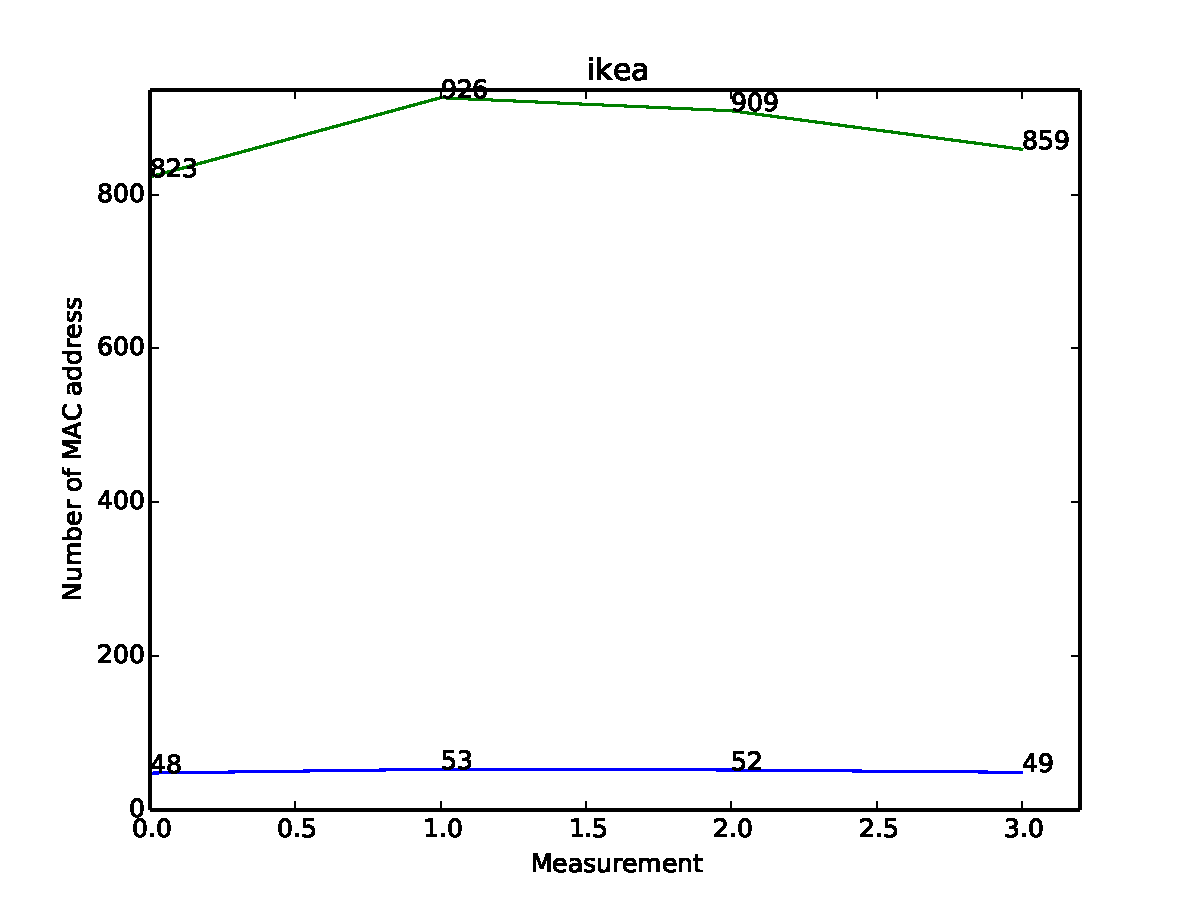
\includegraphics[width=0.9\textwidth]{./ikea-before.pdf}
	\caption{IKEA experiment result before MAC address removal. }
	\label{fig:ikea-before}
\end{figure}

\begin{figure}[H]
	\centering
	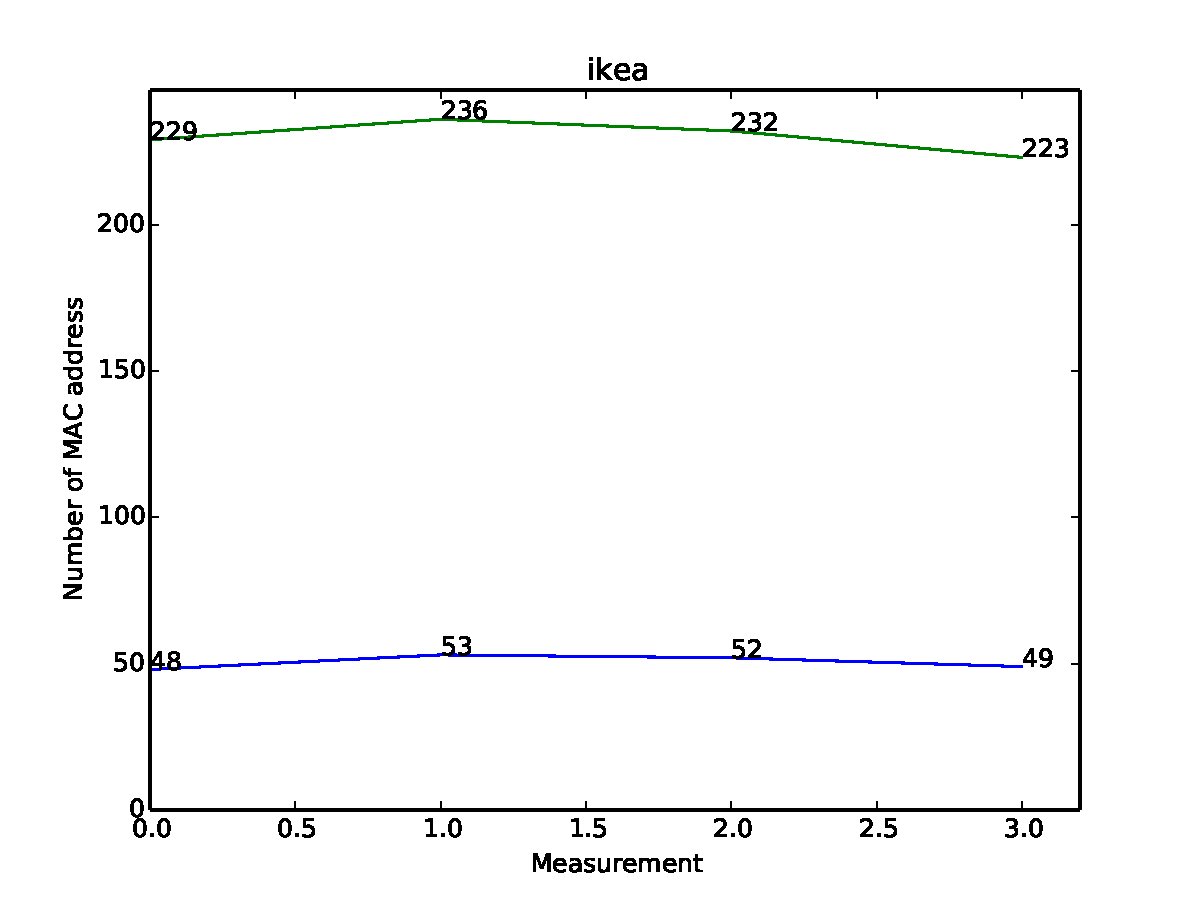
\includegraphics[width=0.9\textwidth]{./ikea.pdf}
	\caption{IKEA experiment result after MAC address removal. }
	\label{fig:ikea-after}
\end{figure}

% subsection ikea_groningen (end)

\subsection{Grotemarkt Groningen} % (fold)
\label{sub:grotemarkt_groningen}
Grotemarkt Groningen is a favorite place for many Groningers in the weekend, which makes this place relatively crowded during weekends. As we can see in Figure~\ref{fig:grotemarkt-before} and~\ref{fig:grotemarkt-after}, the number of devices drop significantly. This is possibly due to this location, which is very dynamic, which has high probability of people going in and out in this area.

\begin{figure}[H]
	\centering
	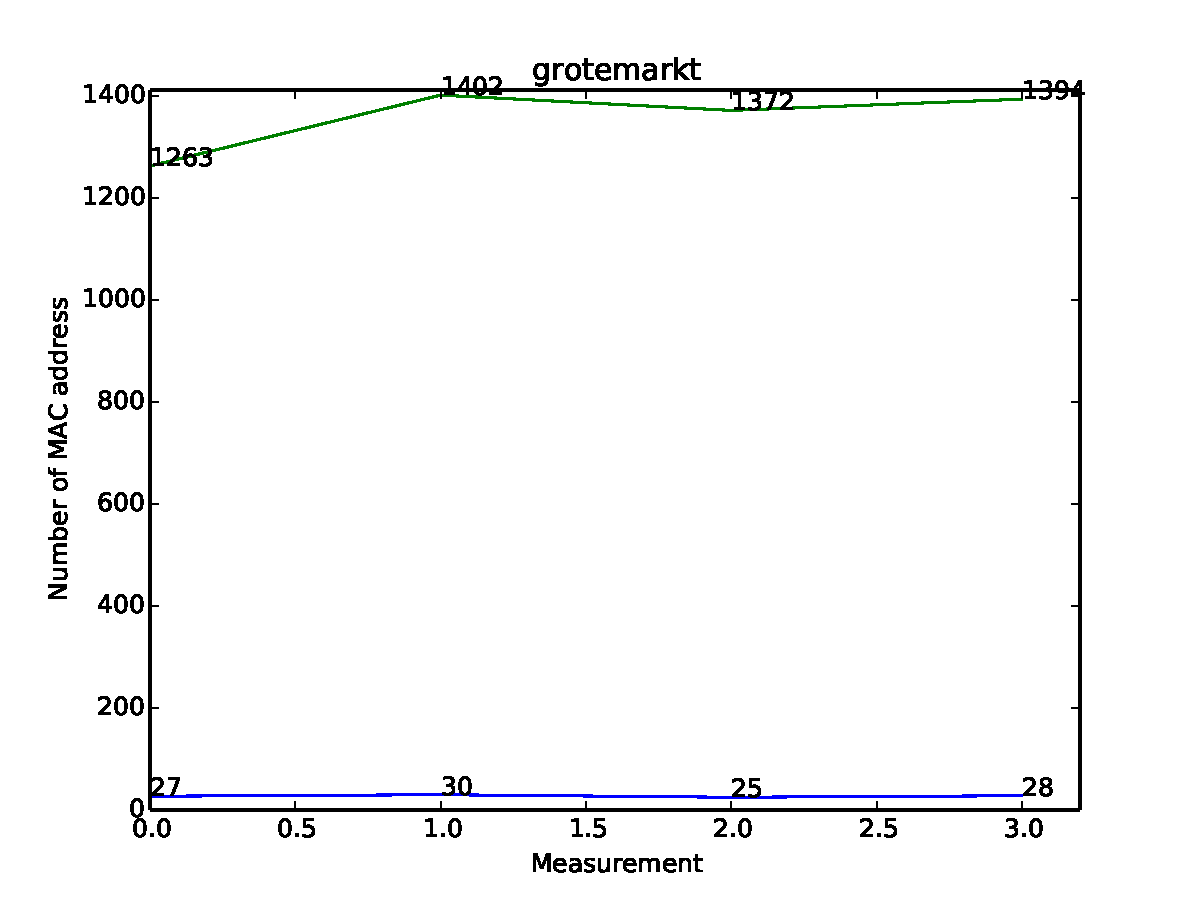
\includegraphics[width=0.9\textwidth]{./grotemarkt-before.pdf}
	\caption{Grotemarkt Groningen experiment result before MAC address removal.}
	\label{fig:grotemarkt-before}
\end{figure}

\begin{figure}[H]
	\centering
	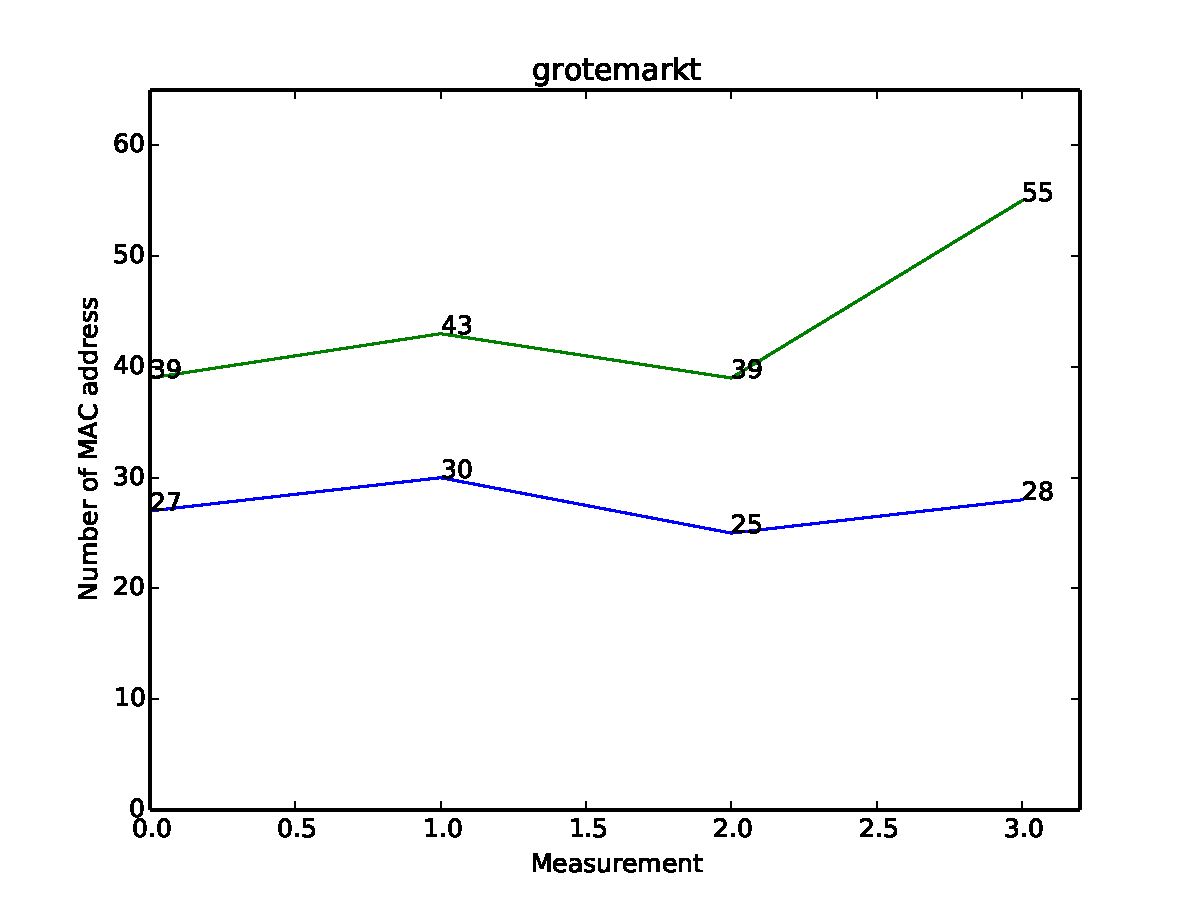
\includegraphics[width=0.9\textwidth]{./grotemarkt.pdf}
	\caption{Grotemarkt Groningen experiment result after MAC address removal. }
	\label{fig:grotemarkt-after}
\end{figure}
% subsection grotemarkt_groningen (end)


\noindent
\textbf{Note:}\\
If we have adequate data, we can present the result in a scatter graph, which could give us clearer correlation overview.
% section result (end)

\bibliography{bibliography}{}
\bibliographystyle{unsrt}
\end{document}